% Copyright (C) 2014-2020 by Thomas Auzinger <thomas@auzinger.name>

\documentclass[draft,final]{vutinfth} % Remove option 'final' to obtain debug information.

% Load packages to allow in- and output of non-ASCII characters.
\usepackage{lmodern}        % Use an extension of the original Computer Modern font to minimize the use of bitmapped letters.
\usepackage[T1]{fontenc}    % Determines font encoding of the output. Font packages have to be included before this line.
\usepackage[utf8]{inputenc} % Determines encoding of the input. All input files have to use UTF8 encoding.

% Extended LaTeX functionality is enables by including packages with \usepackage{...}.
\usepackage{amsmath}    % Extended typesetting of mathematical expression.
\usepackage{amssymb}    % Provides a multitude of mathematical symbols.
\usepackage{mathtools}  % Further extensions of mathematical typesetting.
\usepackage{microtype}  % Small-scale typographic enhancements.
\usepackage[inline]{enumitem} % User control over the layout of lists (itemize, enumerate, description).
\usepackage{multirow}   % Allows table elements to span several rows.
\usepackage{booktabs}   % Improves the typesettings of tables.
\usepackage{subcaption} % Allows the use of subfigures and enables their referencing.
\usepackage[ruled,linesnumbered,algochapter]{algorithm2e} % Enables the writing of pseudo code.
\usepackage[usenames,dvipsnames,table]{xcolor} % Allows the definition and use of colors. This package has to be included before tikz.
\usepackage{nag}       % Issues warnings when best practices in writing LaTeX documents are violated.
\usepackage{todonotes} % Provides tooltip-like todo notes.
\usepackage{hyperref}  % Enables cross linking in the electronic document version. This package has to be included second to last.
\usepackage[acronym,toc]{glossaries} % Enables the generation of glossaries and lists fo acronyms. This package has to be included last.

% Define convenience functions to use the author name and the thesis title in the PDF document properties.
\newcommand{\authorname}{Michael Etschbacher} % The author name without titles.
\newcommand{\thesistitle}{Reducing the operation cost of a file fixity storage service on the ethereum blockchain by utilizing pool testing strategies.} % The title of the thesis. The English version should be used, if it exists.

% Set PDF document properties
\hypersetup{
    pdfpagelayout   = TwoPageRight,           % How the document is shown in PDF viewers (optional).
    linkbordercolor = {Melon},                % The color of the borders of boxes around crosslinks (optional).
    pdfauthor       = {\authorname},          % The author's name in the document properties (optional).
    pdftitle        = {\thesistitle},         % The document's title in the document properties (optional).
    pdfsubject      = {Subject},              % The document's subject in the document properties (optional).
    pdfkeywords     = {a, list, of, keywords} % The document's keywords in the document properties (optional).
}

\setpnumwidth{2.5em}        % Avoid overfull hboxes in the table of contents (see memoir manual).
\setsecnumdepth{subsection} % Enumerate subsections.

\nonzeroparskip             % Create space between paragraphs (optional).
\setlength{\parindent}{0pt} % Remove paragraph identation (optional).

\makeindex      % Use an optional index.
\makeglossaries % Use an optional glossary.
%\glstocfalse   % Remove the glossaries from the table of contents.

% Set persons with 4 arguments:
%  {title before name}{name}{title after name}{gender}
%  where both titles are optional (i.e. can be given as empty brackets {}).
\setauthor{Bsc.}{\authorname}{}{male}
\setadvisor{Ao.univ.Prof. Dr.}{Andreas Rauber}{}{male}

% Required data.
\setregnumber{51828999}
\setdate{01}{01}{2001} % Set date with 3 arguments: {day}{month}{year}.
\settitle{\thesistitle}{\thesistitle} % Sets English and German version of the title (both can be English or German). If your title contains commas, enclose it with additional curvy brackets (i.e., {{your title}}) or define it as a macro as done with \thesistitle.

\setthesis{master}
\setthesis{master}
\setmasterdegree{dipl.} % dipl. / rer.nat. / rer.soc.oec. / master
\setcurriculum{Data Science}{Data Science} % Sets the English and German name of the curriculum.

\begin{document}

\frontmatter % Switches to roman numbering.
% The structure of the thesis has to conform to the guidelines at
%  https://informatics.tuwien.ac.at/study-services

\addtitlepage{naustrian} % German title page (not for dissertations at the PhD School).
\addtitlepage{english} % English title page.
\addstatementpage

\begin{danksagung*}
\todo{Ihr Text hier.}
\end{danksagung*}

\begin{acknowledgements*}
\todo{Enter your text here.}
\end{acknowledgements*}

\begin{kurzfassung}
\todo{Ihr Text hier.}
\end{kurzfassung}

\begin{abstract}
\todo{Enter your text here.}
\end{abstract}

% Select the language of the thesis, e.g., english or naustrian.
\selectlanguage{english}

% Add a table of contents (toc).
\tableofcontents % Starred version, i.e., \tableofcontents*, removes the self-entry.

% Switch to arabic numbering and start the enumeration of chapters in the table of content.
\mainmatter

\chapter{Introduction}

\chapter{Digital Archives}

\chapter{Data Integrity and Authenticity}
\section{Forms of Fixity}
\section{Fixity Checks}
\section{Hashing}
Generally speaking, the purpose of hash functions, in the context of a blockchain, is to compare large datasets quickly and evaluate whether their contents are similar. A one way algorithm processes the entire blocks transactions into 32 bytes of data—a hash, or string, of letters and numbers that contains no discernible information about the transactions within. The hash creates an unmistakable signature for a block, allowing the next block to build on top of it \cite[55]{dannen2017introducing}.

\chapter{Ethereum Blockchain}
\section{Ethereum Blockchain}
\label{sec:eth-blockchain}
Open source blockchain networks such as Ethereum and Bitcoin are kits that allow you to set up an economic system in software, complete with account management, a native unit of exchange to pass between account. These native units of exchange are called coins, tokens, or cryptocurrencies, but the are no different from tokens in any other system: they are a form of money  that is usable only within that system to simply pay your peers or to run programs on the Ethereum network. When you want to make one of these peer-to-peer networks accessible through a web browser, you need to use special software libraries such as Web3.py (used in this thesis)\footnote{\url{https://github.com/ethereum/web3.py}} to connect an applications front end (the GUI you see in a browser), via JavaScript APIs, to its back end (the blockchain) \cite[2]{dannen2017introducing}.
The fact that everyone in the world can interact with the same distributed database, given you have internet access and a decent device, is favoritable in the case of an fixity storage as presented in \ref{chapter:fixity_storage} since anyone will be able to confirm if an object has changed over time. Lets say an digital archive releases multiple objects to the public and their respective fixity information on the blockchain, citizens could then validate if the object in question is really what it is meant to be. Trust in the archive is therefore not needed anymore, which will strenghten the general trust of the archive.
A block is a unit of time that encompasses a certain number of transactions. Inside that period, transaction data is recorded; when the unit of time elapses, the next block begins. The blockchain represents the history of state changes within the network database of the EVM \cite[43]{dannen2017introducing}.
Transactions and state changes in the Ethereum network are segmented into blocks, and then hashed. Each block is verified and validated before the next canonical block can be placed on top of it. In this way, nodes on the network do not need to individually evaluate the trustworthiness of every single block in the history of the Ethereum network, simply to compute the present balances of the accounts on the network. They merely verify that its “parent block” is the most recent canonical block. They do this quickly by looking to see that the new block contains the correct hash of its parents transactions and state. All the blocks strung together, and including the genesis block, an honorific describing the first block the network mined after coming online, are called the blockchain. In some circles, you will hear the blockchain referred to as a distributed ledger or distributed ledger technology (DLT). Ledger is an accurate description, as the chain contains every transaction in the history of the network, making it effectively a giant, balanced book of accounts \cite[55]{dannen2017introducing}. 
\section{Ethereum Virtual Machine}
\label{sec:evm}
The EVMs physical instantiation can not be described in the same way that one might point to a cloud or an ocean wave, but it does exist as one single entity maintained by thousands of connected computers running an Ethereum client \footnote{\url{https://ethereum.org/en/developers/docs/evm/}}.
A virtual machine (VM), in the Ethereum context, is one giant global computer composed of constituent nodes, which are themselves computers too. Generally speaking, a virtual machine is an emulation of a computer system by another computer system. These emulations are based on the same computer architectures as the target of their emulation, but they are usually reproducing that architecture on different hardware than it may have been intended for. Virtual machines can be created with hardware, software, or both. In the case of Ethereum, it is both. Rather than securely network thousands of discrete machines, Ethereum takes the approach of securely operating one very large state machine that can encompass the whole Earth \cite[48]{dannen2017introducing}.
The EVM can run arbitrary computer programs written in the Solidity\footnote{\url{https://github.com/ethereum/solidity}} language. These programs, given a particular input, will always produce the output the same way, with the same underlying state changes. This makes Solidity programs fully deterministic and guaranteed to execute, provided youve paid enough for the transaction. Solidity programs are capable of expressing all tasks accomplishable by computers, making them theoretically Turing complete. That means that the entire distributed network, every node, performs every program executed on the platform \cite[50]{dannen2017introducing}. 
From the perspective of a software developer, the EVM is also a runtime environment for small programs that can be executed by the network. The EVM has its own language, the EVM bytecode, to which your smart contracts compile. Solidity, which is a high-level language, is compiled into bytecode and uploaded onto the Ethereum blockchain by using a client application such as geth\footnote{\url{https://geth.ethereum.org/}} \cite[51]{dannen2017introducing}.
\section{Gas and Fees}
Gas refers to the unit that measures the amount of computational effort required to execute specific operations on the Ethereum network. Since each Ethereum transaction requires computational resources to execute, each transaction requires a fee. Gas refers to the fee required to conduct a transaction on Ethereum successfully.
Gas fees are paid in Ethereum's native currency, ether (ETH). Gas prices are denoted in gwei, which itself is a denomination of ETH - each gwei is equal to 0.000000001 ETH (10-9 ETH). For example, instead of saying that your gas costs 0.000000001 ether, you can say your gas costs 1 gwei. The word 'gwei' itself means 'giga-wei', and it is equal to 1,000,000,000 wei. Wei itself is the smallest unit of ETH\footnote{\url{https://ethereum.org/en/developers/docs/gas/}}.
\section{Smart Contracts}
Smart contracts are the building blocks of decentralized applications running on the EVM, they are like the concept of classes in conventional object-oriented programming. When developers speak of writing smart contracts, they are typically referring to the practice of writing code in the Solidity language to be executed on the Ethereum network. When the code is executed, units of value may be transferred as easily as data \cite[10]{dannen2017introducing}.
In my thesis, the fixity storage is often referenced as decentralized application (DAPP) which is built with several smart contracts. The main smart contract used in this thesis is further described in Section \ref{chapter:fixity_storage}. 

\section{Persistence}
Unlike a centralized server operated by a single company or organization, decentralized storage systems consist of a peer-to-peer network of user-operators who hold a portion of the overall data, creating a resilient file storage sharing system. These can be in a blockchain-based application or any peer-to-peer-based network. Ethereum itself can be used as a decentralized storage system, and it is when it comes to code storage in all the smart contracts. However, when it comes to large amounts of data, that isn't what Ethereum was designed for. The chain is steadily growing, but at the time of writing, the Ethereum chain is 602.95 GB for Mar 19 2022\footnote{\url{https://ycharts.com/indicators/ethereum_chain_full_sync_data_size}}, and every node on the network needs to be able to store all of the data. If the chain were to expand to large amounts of data (say 5TBs) it wouldn't be feasible for all nodes to continue to run. Also, the cost of deploying this much data to Mainnet would be prohibitively expensive due to gas fees \footnote{\url{https://ethereum.org/en/developers/docs/storage/}}.
My proposed solution using pooled testing, presented in Section \ref{chapter:pooled_testing}, counters the ever increasing chain size of the Ethereum network by reducing the amount of write transaction by at least 50 percent. Each writing transaction performed from the fixity storage stores exactly one sha256 result, on the blockchain. The gas cost of storing 256 bit on the blockchain can be read from Table \ref{table:gas-costs}.
All transactions in Ethereum are stored on the blockchain, a canonical history of state changes stored on every single Ethereum node \cite[12]{dannen2017introducing}.
Like all databases, a blockchain has a schema: rules define, constrain, and enforce relationships between entities. Motivations to break or alter these relationships can be found across industries, leading to bribery and corruption, and making blockchains trustless qualities even more attractive to business than prior generations of software and networking. In all databases, shared read/write access creates enormous complexity. Machines all over the world may experience varying latency, depending on where the database is physically located, leading to some write operations arriving out of order. This gets even more difficult if several parties are supposed to equally share a database \cite[20]{dannen2017introducing}. 
The nodes go through the block they are process and run any code enclosed within the transactions. Each node does this independently; it is not only highly parallelized, but highly redundant. Despite the high redundany, this is an efficient way to balance a global ledger in a trustworthy way \cite[50]{dannen2017introducing}.
\subsection{Blockchain-based persistence}
This type of persistence is utilized in my thesis, since the fixity information of the archived objects are meant to be persisted for longterm.
For a piece of data to persist forever, Ethereum needs to use a persistence mechanism. For example, on Ethereum, the persistence mechanism is that the whole chain needs to be accounted for when running a node. New pieces of data get tacked onto the end of the chain, and it continues to grow - requiring every node to replicate all the embedded data. This is known as blockchain-based persistence. The issue with blockchain-based persistence is that the chain could get far too big to upkeep and store all the data feasibly (e.g. many sources estimate the Internet to require over 40 Zetabytes of storage capacity). The blockchain must also have some type of incentive structure. For blockchain-based persistence, there is a payment made to the miner. When the data is added to the chain, the nodes are paid to add the data on \footnote{\url{https://ethereum.org/en/developers/docs/storage/}}.
\subsection{Contract-based persistence}
Contract-based persistence has the intuition that data cannot be replicated by every node and stored forever, and instead must be upkept with contract agreements. These are agreements made with multiple nodes that have promised to hold a piece of data for a period of time. They must be refunded or renewed whenever they run out to keep the data persisted. In most cases, instead of storing all data on-chain, the hash of where the data is located on a chain gets stored. This way, the entire chain doesn't need to scale to keep all of the data \footnote{\url{https://ethereum.org/en/developers/docs/storage/}}.
\section{Test Networks}. 
These networks are not really free of charge, but the ether token on the respective network is free to get. Although the queue of the free ether token can be very vast in some cases e.g. https://faucet.dimensions.network/ this faucet has a waiting queue for over three days until you recieve one ether token for the ropsten network. Other faucets, a distributer of free ether test tokens, require social network accounts to verifiy that you are not a bot e.g. https://faucet.paradigm.xyz/ requires a twitter account with at least one tweet and at least 15 retweets before you can request one ether token. The faucet request are almost all time gated, meaning that you could request ether only once per day. At small scale, this limitation is no problem for this thesis because persisting around 10 pools on the blockchains require at max 0.002 ether tokens. The one per day paradigm gets problemeatic for the experiment for the 10.000 objects, which costs about 20 ether tokens, which means I would have to request tokens fors 20 days straight to perform one experiment on a real live environment such as the ropsten testnetwork. 
There are multiple options to choose from for a testnetwork, from the most prominent networks presented at the official ethereum documentation https://ethereum.org/en/developers/docs/networks/ only the ropsten network implements the proof-of-work algorithm, which means it is the best representation of ethereum to date, and for that reason I decided to utilize the ropsten network in this experiment
\section{Costs}
\label{sec:costs}
Miners are paid this ether for mining, and also for running scripts on the network. The cost associated with electricity expenditure of servers running on the Ethereum network is one of the factors that gives ether, as a cryptocommodity, its intrinsic value—that is, someone paid real money to their electricity company to run their mining machine. Specialized mining rigs, which use arrays of graphics cards to increase their odds of completing a block and getting paid \cite[12]{dannen2017introducing}. 
Mining achieves the consensus required to make valid state changes, and the miners are paid for contributing to the consensus building. This is how ether and bitcoin are created  \cite[57]{dannen2017introducing}. 
For every instruction the EVM executes, there must be a cost associated, to ensure the system isnt jammed up by useless spam contracts. Every time an instruction executes, an internal counter keeps track of the fees incurred, which are charged to the user. Each time the user initiates a transaction, that users wallet reserves a small portion to pay these fees \cite[58]{dannen2017introducing}. The fees are the driving factor of my thesis where I try to make as less transactions as possible to run a fixity storage system on the Ethereum network. 
The fees are dependent on the gas cost of a transaction, gas is a unit of work; it is not a subcurrency, and you can not hold or hoard it. It simply measures how much effort each step of a transaction will be, in computational terms. To be able to pay for gas costs, you simply need to add ether to your account. You do not have to acquire it separately; there is no gas token. Every operation possible on the EVM has an associated gas cost. Gas costs ensure that computation time on the network is appropriately priced \cite[59]{dannen2017introducing}.
If you send a computationally difficult set of instructions to the EVM, the only person this hurts is you. The work will spend your ether, and stop when the ether you allocated to the transaction runs out. It has no effect on anyone elses transactions. There is no way to jam up the EVM without paying a lot, in the form of transaction fees, to do it. Scaling is handled in a de facto way through the gas fee system. Miners are free to choose the transactions that pay the highest fee rates, and can also choose the block gas limit collectively. The gas limit determines how much computation can happen (and how much storage can be allocated) per block \cite[60]{dannen2017introducing}. 
\section{Transactions}
An Ethereum transaction refers to an action initiated by an externally-owned account, in other words an account managed by a human, not a contract. For example, if Bob sends Alice 1 ETH, Bob's account must be debited and Alice's must be credited. This state-changing action takes place within a transaction. 
\begin{figure}[h]
    \caption{Illustration of an ethereum transaction \url{https://ethereum.org/en/developers/docs/transactions/}}
    \centering
    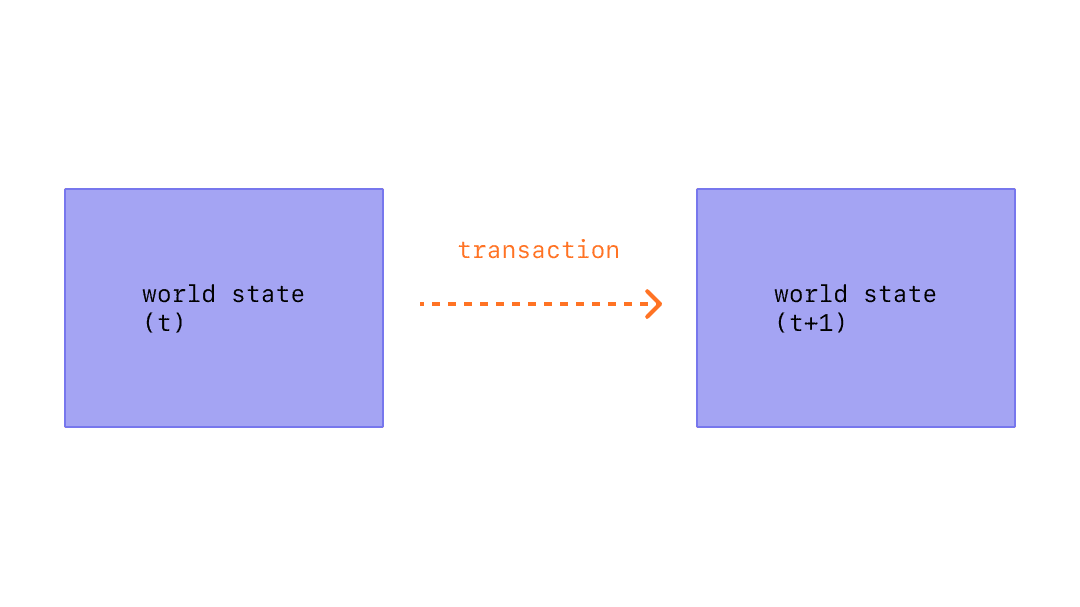
\includegraphics[width=0.5\textwidth]{eth_transaction.png}
\end{figure}
Transactions, which change the state of the EVM, need to be broadcast to the whole network. Any node can broadcast a request for a transaction to be executed on the EVM; after this happens, a miner will execute the transaction and propagate the resulting state change to the rest of the network. \footnote{\url{https://ethereum.org/en/developers/docs/transactions/}}.
\begin{verbatim}
{
  from: "0xAF8725604990d46042A50EfD9e2cB118141Bb140",
  to: "0x2C3c7752cE837bB97D6C31B4f883EAAA92BC3Ce5",
  gasLimit: "21000",
  maxFeePerGas: "300",
  maxPriorityFeePerGas: "10",
  nonce: "42",
  value: "10000000000"
}
\end{verbatim}
Transactions come from external accounts, which are usually controlled by human users. It is a way for an external account to submit instructions to the EVM to perform some operation. In other words, it is a way for an external account to get a message into the system. A transaction in the EVM is a cryptographically signed data package storing a message, which tells the EVM to transfer ether, create a new contract, trigger an existing one, or perform some calculation. Contract addresses can be the recipients of transactions, just like users with external accounts \cite[60]{dannen2017introducing}. 
Table \ref{table:gas-costs} presents the gas cost of the most used operation used in this thesis according to the Ethereum yellow paper \cite[27]{wood2014ethereum}.
\begin{center}
    \begin{tabular}{ c c c }\label{table:gas-costs}
     Operation Name & Gas Cost & Description \\ 
     $G_codedeposit$ & 200 & gas cost per bytesize of the compiled bytecode of the smart contract \\  
     $G_txcreate$ & 32000 & create a new smart contract  \\   
     $G_transaction$ & 21000 & retrieve the current balance of an account \\
     $G_txdatanonzero$ & 16 & gas cost per bytesize of the compiled bytecode of the transaction  \\   
     $G_balance$ & 400 & retrieve the current balance of an account 
    \end{tabular}
\end{center}
\section{Events}
\label{sec:events}

\chapter{Fixity Storage}

\chapter{Pooling Strategy}

\chapter{Experiment}

\chapter{Evaluation}

\chapter{Discussion}

\chapter{Conclusion}

\chapter{Related Work}

% Remove following line for the final thesis.
%%% intro.tex
%% Copyright (C) 2014-2020 by Thomas Auzinger <thomas@auzinger.name>
%
% This work may be distributed and/or modified under the
% conditions of the LaTeX Project Public License, either version 1.3
% of this license or (at your option) any later version.
% The latest version of this license is in
%   http://www.latex-project.org/lppl.txt
% and version 1.3 or later is part of all distributions of LaTeX
% version 2005/12/01 or later.
%
% This work has the LPPL maintenance status `maintained'.
%
% The Current Maintainer of this work is Thomas Auzinger.
%
% This work consists of the files vutinfth.dtx and vutinfth.ins
% and the derived file vutinfth.cls.
% This work also consists of the file intro.tex.


\newacronym{ctan}{CTAN}{Comprehensive TeX Archive Network}
\newacronym{faq}{FAQ}{Frequently Asked Questions}
\newacronym{pdf}{PDF}{Portable Document Format}
\newacronym{svn}{SVN}{Subversion}
\newacronym{wysiwyg}{WYSIWYG}{What You See Is What You Get}

\newglossaryentry{texteditor}
{
  name={editor},
  description={A text editor is a type of program used for editing plain text files.}
}

\chapter{Introduction to \LaTeX}

Since \LaTeX\ is widely used in academia and industry, there exists a plethora of freely accessible introductions to the language.
Reading through the guide at \url{https://en.wikibooks.org/wiki/LaTeX} serves as a comprehensive overview for most of the functionality and is highly recommended before starting with a thesis in \LaTeX.

\section{Installation}

A full \LaTeX\ distribution\index{distribution} consists not only of the binaries that convert the source files to the typeset documents, but also of a wide range of packages and their documentation.
Depending on the operating system, different implementations are available as shown in Table~\ref{tab:distrib}.
\textbf{Due to the large amount of packages that are in everyday use and due to their high interdependence, it is paramount to keep the installed distribution\index{distribution} up to date.}
Otherwise, obscure errors and tedious debugging ensue.

\begin{table}
  \centering
  \begin{tabular}{cccc}
    \toprule
    Distribution & Unix         & Windows      & MacOS        \\
    \midrule
    TeX Live     & \textbf{yes} & yes          & (yes)        \\
    MacTeX       & no           & no           & \textbf{yes} \\
    MikTeX       & (yes)        & \textbf{yes} & yes          \\
    \bottomrule
  \end{tabular}
  \caption{\TeX/\LaTeX\ distributions for different operating systems. Recomended choice in \textbf{bold}.}
  \label{tab:distrib} % \label has to be placed AFTER \caption to produce correct cross-references.
\end{table}

\section{Editors}

A multitude of \TeX\ \glspl{texteditor} are available differing in their editing models, their supported operating systems and their feature sets.
A comprehensive overview of \glspl{texteditor} can be found at the Wikipedia page  \url{https://en.wikipedia.org/wiki/Comparison_of_TeX_editors}.
TeXstudio (\url{http://texstudio.sourceforge.net/}) is recommended.
Most editors support a synchronization of the generated document and the \LaTeX\ source by \verb|Ctrl| clicking either on the source document or the generated document.

\section{Compilation}

Modern editors usually provide the compilation programs to generate \gls{pdf} documents and for most \LaTeX\ source files, this is sufficient.
More advanced \LaTeX\ functionality, such as glossaries and bibliographies, needs additional compilation steps, however.
It is also possible that errors in the compilation process invalidate intermediate files and force subsequent compilation runs to fail.
It is advisable to delete intermediate files (\verb|.aux|, \verb|.bbl|, etc.), if errors occur and persist.
All files that are not generated by the user are automatically regenerated.
To compile the current document, the steps as shown in Table~\ref{tab:compile} have to be taken.


\begin{table}
  \centering
  \begin{tabular}{rl}
    \toprule
    & Description \\
    \midrule
    1 & Scan for refs, toc/lof/lot/loa items and cites \\
    2 & Build the bibliography     \\
    3 & Link refs and build the toc/lof/lot/loa \\
    4 & Link the bibliography \\
    5 & Build the glossary \\
    6 & Build the acronyms \\
    7 & Build the index \\
    8 & Link the glossary, acronyms, and the index \\
    9 & Link the bookmarks \\
    \midrule
    & Command \\
    \midrule
    1 & \verb|pdflatex.exe  example| \\
    2 & \verb|bibtex.exe    example| \\
    3 & \verb|pdflatex.exe  example| \\
    4 & \verb|pdflatex.exe  example| \\
    5 & \verb|makeindex.exe -t example.glg -s example.ist| \\
      & \verb|              -o example.gls example.glo| \\
    6 & \verb|makeindex.exe -t example.alg -s example.ist| \\
      & \verb|              -o example.acr example.acn| \\
    7 & \verb|makeindex.exe -t example.ilg -o example.ind example.idx| \\
    8 & \verb|pdflatex.exe  example| \\
    9 & \verb|pdflatex.exe  example| \\
    \bottomrule
  \end{tabular}
  \caption{Compilation steps for this document. The following abbreviations were used: table of contents (toc), list of figures (lof), list of tables (lot), list of algorithms (loa).}
  \label{tab:compile} % \label has to be placed AFTER \caption to produce correct cross-references.
\end{table}


\section{Basic Functionality}

In this section, various examples are given of the fundamental building blocks used in a thesis.
Many \LaTeX\ commands have a rich set of options that can be supplied as optional arguments.
The documentation of each command should be consulted to get an impression of the full spectrum of its functionality.

\subsection{Floats}

Two main categories of page elements can be differentiated in the usual \LaTeX\ workflow: \textit{(i)} the main stream of text and \textit{(ii)} floating containers that are positioned at convenient positions throughout the document.
In most cases, tables, plots, and images are put into such containers since they are usually positioned at the top or bottom of pages.
These are realized by the two environments \verb|figure| and \verb|table|, which also provide functionality for cross-referencing (see Table~\ref{tab:intro} and Figure~\ref{fig:intro}) and the generation of corresponding entries in the list of figures and the list of tables.
Note that these environments solely act as containers and can be assigned arbitrary content.

\subsection{Tables}

A table in \LaTeX\ is created by using a \verb|tabular| environment or any of its extensions, e.g., \verb|tabularx|.
The commands \verb|\multirow| and \verb|\multicolumn| allow table elements to span multiple rows and columns.

\begin{table}[h] % placement specifier
  \centering
  \begin{tabular}{lll}
    \toprule
    \multicolumn{2}{c}{Position} \\
    \cmidrule{1-2} % partial horizontal rule
    Group & Abbrev & Name \\
    \midrule
    Goalkeeper & GK & Paul Robinson \\
    \midrule
    \multirow{4}{*}{Defenders} & LB & Lucus Radebe \\
                               & DC & Michael Duburry \\
                               & DC & Dominic Matteo \\
                               & RB & Didier Domi \\
    \midrule
    \multirow{3}{*}{Midfielders} & MC & David Batty \\
                                 & MC & Eirik Bakke \\
                                 & MC & Jody Morris \\
    \midrule
    Forward & FW & Jamie McMaster \\
    \midrule
    \multirow{2}{*}{Strikers} & ST & Alan Smith \\
                              & ST & Mark Viduka \\
    \bottomrule
  \end{tabular}
  \caption{Adapted example from the \LaTeX guide at \url{https://en.wikibooks.org/wiki/LaTeX/Tables}. This example uses rules specific to the \texttt{booktabs} package and employs the multi-row functionality of the \texttt{multirow} package.}
  \label{tab:intro} % \label has to be placed AFTER \caption to produce correct cross-references.
\end{table}

\subsection{Images}

An image is added to a document via the \verb|\includegraphics| command as shown in Figure~\ref{fig:intro}.
The \verb|\subcaption| command can be used to reference subfigures, such as Figure~\ref{fig:intro:full width} and~\ref{fig:intro:half width}.

\begin{figure}[h]
  \centering
  \begin{subfigure}[b]{0.45\columnwidth}
    \centering
    
\includegraphics[width=\textwidth]{Logo-schwarz.pdf}
    \subcaption{The header logo at text width.}
    \label{fig:intro:full width}
  \end{subfigure}
  \begin{subfigure}[b]{0.45\columnwidth}
    \centering
    
\includegraphics[width=0.5\textwidth]{Logo-schwarz.pdf}
    \subcaption{The header logo at half the text width.}
    \label{fig:intro:half width}
  \end{subfigure}
  \caption[Optional caption for the figure list (often used to abbreviate long captions)]{The header logo at different sizes.} % Remove the [...] argument if the original caption should be used in the figure list.
  \label{fig:intro} % \label has to be placed AFTER \caption (or \subcaption) to produce correct cross-references.
\end{figure}

\subsection{Mathematical Expressions}

One of the original motivation to create the \TeX\ system was the need for mathematical typesetting.
To this day, \LaTeX\ is the preferred system to write math-heavy documents and a wide variety of functions aids the author in this task.
A mathematical expression can be inserted inline as $\sum_{n=1}^{\infty} \frac{1}{n^2} = \frac{\pi^2}{6}$ outside of the text stream as \[ \sum_{n=1}^{\infty} \frac{1}{n^2} = \frac{\pi^2}{6} \] or as numbered equation with
\begin{equation}
\sum_{n=1}^{\infty} \frac{1}{n^2} = \frac{\pi^2}{6}.
\end{equation}

\subsection{Pseudo Code}

The presentation of algorithms can be achieved with various packages; the most popular are \verb|algorithmic|, \verb|algorithm2e|, \verb|algorithmicx|, or \verb|algpseudocode|.
An overview is given at \url{https://tex.stackexchange.com/questions/229355}.
An example of the use of the \verb|alogrithm2e| package is given with Algorithm~\ref{alg:gauss-seidel}.

\begin{algorithm}
  \SetKw{BreakFor}{break for}
  \KwIn{A scalar~$\epsilon$, a matrix $\mathbf{A} = (a_{ij})$, a vector $\vec{b}$, and an initial vector $\vec{x}^{(0)}$}
  \KwOut{$\vec{x}^{(n)}$ with $\mathbf{A} \vec{x}^{(n)} \approx \vec{b}$}
  \For{$k\leftarrow 1$ \KwTo maximum iterations}
  {
     \For{$i\leftarrow 1$ \KwTo $n$}
     {
        $x_i^{(k)} = \frac{1}{a_{ii}} \left(b_i-\sum_{j<i} a_{ij} x_j^{(k)} - \sum_{j>i} a_{ij} x_j^{(k-1)} \right)$\;
     }
     \If{$\lvert\vec{x}^{(k)}-\vec{x}^{(k-1)}\rvert < \epsilon$}
     {\BreakFor\;}
  }
  \Return{$\vec{x}^{(k)}$\;}
  \caption{Gauss-Seidel}
  \label{alg:gauss-seidel} % \label has to be placed AFTER \caption to produce correct cross-references.
\end{algorithm}

\section{Bibliography}

The referencing of prior work is a fundamental requirement of academic writing and well supported by \LaTeX.
The \textsc{Bib}\TeX\ reference management software is the most commonly used system for this purpose.
Using the \verb|\cite| command, it is possible to reference entries in a \verb|.bib| file out of the text stream, e.g., as~\cite{Turing1936}.
The generation of the formatted bibliography needs a separate execution of \verb|bibtex.exe| (see Table~\ref{tab:compile}).

\section{Table of Contents}

The table of contents is automatically built by successive runs of the compilation, e.g., of \verb|pdflatex.exe|.
The command \verb|\setsecnumdepth| allows the specification of the depth of the table of contents and additional entries can be added to the table of contents using \verb|\addcontentsline|.
The starred versions of the sectioning commands, i.e., \verb|\chapter*|, \verb|\section*|, etc., remove the corresponding entry from the table of contents.

\section{Acronyms / Glossary / Index}

The list of acronyms, the glossary, and the index need to be built with a separate execution of \verb|makeindex| (see Table~\ref{tab:compile}).
Acronyms have to be specified with \verb|\newacronym| while glossary entries use \verb|\newglossaryentry|.
Both are then used in the document content with one of the variants of \verb|\gls|, such as \verb|\Gls|, \verb|\glspl|, or \verb|\Glspl|.
Index items are simply generated by placing \verb|\index|\marg{entry} next to all the words that correspond to the index entry \meta{entry}.
Note that many enhancements exist for these functionalities and the documentation of the \verb|makeindex| and the \verb|glossaries| packages should be consulted.

\section{Tips}

Since \TeX\ and its successors do not employ a \gls{wysiwyg} editing scheme, several guidelines improve the readability of the source content:
\begin{itemize}
\item Each sentence in the source text should start with a new line.
      This helps not only the user navigation through the text, but also enables revision control systems (e.g. \gls{svn}, Git) to show the exact changes authored by different users.
      Paragraphs are separated by one (or more) empty lines.
\item Environments, which are defined by a matching pair of \verb|\begin{name}| and \verb|\end{name}|, can be indented by whitespace to show their hierarchical structure.
\item In most cases, the explicit use of whitespace (e.g. by adding \verb|\hspace{4em}| or \verb|\vspace{1.5cm}|) violates typographic guidelines and rules.
      Explicit formatting should only be employed as a last resort and, most likely, better ways to achieve the desired layout can be found by a quick web search.
\item The use of bold or italic text is generally not supported by typographic considerations and the semantically meaningful \verb|\emph{|\texttt{$\dots$}\verb|}| should be used.
\end{itemize}

The predominant application of the \LaTeX\ system is the generation of \gls{pdf} files via the \textsc{Pdf}\LaTeX\ binaries.
In the current version of \textsc{Pdf}\LaTeX, it is possible that absolute file paths and user account names are embedded in the final \gls{pdf} document.
While this poses only a minor security issue for all documents, it is highly problematic for double blind reviews.
The process shown in Table~\ref{tab:ps2pdf} can be employed to strip all private information from the final \gls{pdf} document.

\begin{table}[h]
  \centering
  \begin{tabular}{rl}
  \toprule
  & Command \\
  \midrule
  1 & Rename the \gls{pdf} document \verb|final.pdf| to \verb|final.ps|. \\
  2 & Execute the following command: \\
    & \verb|ps2pdf -dPDFSETTINGS#/prepress ^| \\
    & \verb| -dCompatibilityLevel#1.4 ^| \\
    & \verb| -dAutoFilterColorImages#false ^| \\
    & \verb| -dAutoFilterGrayImages#false ^| \\
    & \verb| -dColorImageFilter#/FlateEncode ^| \\
    & \verb| -dGrayImageFilter#/FlateEncode ^| \\
    & \verb| -dMonoImageFilter#/FlateEncode ^| \\
    & \verb| -dDownsampleColorImages#false ^| \\
    & \verb| -dDownsampleGrayImages#false ^| \\
    & \verb| final.ps final.pdf| \\
  \bottomrule
  \end{tabular}

  On Unix-based systems, replace \verb|#| with \verb|=| and \verb|^| with \verb|\|.
  \caption{Anonymization of \gls{pdf} documents.}
  \label{tab:ps2pdf}
\end{table}

\section{Resources}

\subsection{Useful Links}

In the following, a listing of useful web resources is given.
\begin{description}
\item[\url{https://en.wikibooks.org/wiki/LaTeX}] An extensive wiki-based guide to \LaTeX.
\item[\url{http://www.tex.ac.uk/faq}] A (huge) set of \gls{faq} about \TeX\ and \LaTeX.
\item[\url{https://tex.stackexchange.com/}] The definitive user forum for non-trivial \LaTeX-related questions and answers.
\end{description}

\subsection[Comprehensive TeX Archive Network]{\gls{ctan}}

The \gls{ctan} is the official repository for all \TeX\ related material.
It can be accessed via \url{https://www.ctan.org/} and hosts (among other things) a huge variety of packages that provide extended functionality for \TeX\ and its successors.
Note that most packages contain \gls{pdf} documentation that can be directly accessed via \gls{ctan}.

In the following, a short, non-exhaustive list of relevant \gls{ctan}-hosted packages is given together with their relative path.
\begin{description}[itemsep=0ex]
\item[\href{https://www.ctan.org/pkg/algorithm2e}{algorithm2e}] Functionality for writing pseudo code.
\item[\href{https://www.ctan.org/pkg/amsmath}{amsmath}] Enhanced functionality for typesetting mathematical expressions.
\item[\href{https://www.ctan.org/pkg/amsfonts}{amssymb}] Provides a multitude of mathematical symbols.
\item[\href{https://www.ctan.org/pkg/booktabs}{booktabs}] Improved typesetting of tables.
\item[\href{https://www.ctan.org/pkg/enumitem}{enumitem}] Control over the layout of lists (\verb|itemize|, \verb|enumerate|, \verb|description|).
\item[\href{https://www.ctan.org/pkg/fontenc}{fontenc}] Determines font encoding of the output.
\item[\href{https://www.ctan.org/pkg/glossaries}{glossaries}] Create glossaries and list of acronyms.
\item[\href{https://www.ctan.org/pkg/graphicx}{graphicx}] Insert images into the document.
\item[\href{https://www.ctan.org/pkg/inputenc}{inputenc}] Determines encoding of the input.
\item[\href{https://www.ctan.org/pkg/l2tabu}{l2tabu}] A description of bad practices when using \LaTeX.
\item[\href{https://www.ctan.org/pkg/mathtools}{mathtools}] Further extension of mathematical typesetting.
\item[\href{https://www.ctan.org/pkg/memoir}{memoir}] The document class on upon which the \verb|vutinfth| document class is based.
\item[\href{https://www.ctan.org/pkg/multirow}{multirow}] Allows table elements to span several rows.
\item[\href{https://www.ctan.org/pkg/pgfplots}{pgfplots}] Function plot drawings.
\item[\href{https://www.ctan.org/pkg/pgf}{pgf/TikZ}] Creating graphics inside \LaTeX\ documents.
\item[\href{https://www.ctan.org/pkg/subcaption}{subcaption}] Allows the use of subfigures and enables their referencing.
\item[\href{https://www.ctan.org/tex-archive/info/symbols/comprehensive/}{symbols/comprehensive}] A listing of around 5000 symbols that can be used with \LaTeX.
\item[\href{https://www.ctan.org/pkg/voss-mathmode}{voss-mathmode}] A comprehensive overview of typesetting mathematics in \LaTeX.
\item[\href{https://www.ctan.org/pkg/xcolor}{xcolor}] Allows the definition and use of colors.
\end{description} % A short introduction to LaTeX.

\backmatter

% Use an optional list of figures.
%\listoffigures % Starred version, i.e., \listoffigures*, removes the toc entry.

% Use an optional list of tables.
%\cleardoublepage % Start list of tables on the next empty right hand page.
%\listoftables % Starred version, i.e., \listoftables*, removes the toc entry.

% Use an optional list of alogrithms.
%\listofalgorithms
%\addcontentsline{toc}{chapter}{List of Algorithms}

% Add an index.
\printindex

% Add a glossary.
\printglossaries

% Add a bibliography.
\bibliographystyle{alpha}
\bibliography{bibliography}
\todo{Enter your text here.}
\end{document}